\section{Durchf\"{u}hrung}

Die Myonen, deren Lebensdauer gemessen werden sollen, entstehen aus Pion- und Kaonzerfällen, die durch Wechselwirkung von Atmosphärenteilchen mit kosmischer Strahlung gebildet werden. Aufgrund ihrer relativistischen Energie erreichen sie den Erdboden. Durch Wechselwirkung mit Materie geben sie einen Teil ihrer kinetischen Energie ab. Bei Durchgang durch einen Szintillator in einem Edelstahltank regt die abgegebene Energie das Szintillatormaterial an, sodass bei der Rückkehr in den Grundzustand Photonen im kurzwelligen sichtbaren bis UV-Bereich emittiert werden. Diese Photonen werden mit zwei Sekundärelektronenvervielfachern (SEV) detektiert, die an den Enden des Tanks angebracht sind. Niederenergetische Myonen können innerhalb des Detektionsvolumen in ein Elektron zerfallen, welches ebenfalls durch einen Lichtblitz einen Strompuls in den SEVs auslöst. Der zeitliche Abstand zwischen dem Myon- und dem Elektronsignal ist dann die Lebensdauer des Myons im Tank.

Ein Lichtblitz entsteht also zum Einen dadurch, dass ein Myon in das Detektionsvolumen eintritt und zum Anderen dadurch, dass ein Myon zerfällt. Die ausgelösten Signale können durch das Messverfahren mit den SEVs nicht unterschieden werden. Als Basis für die Messung der Lebensdauer wird davon ausgegangen, dass der zeitliche Abstand zweier in den Tank eindringenden Myonen größer ist, als die Zerfallszeit eines Myons. Ein Lichtblitz wird also als Startpuls definiert. Wenn ein weiterer Lichtblitz innerhalb der Suchzeit $T_\text{S}$ auf das Startsignal folgt, wird dieser als Stopppuls für die Zeitmessung definiert und die Zeitdifferenz als Messwert für die Lebensdauer verwendet. Ist der Lichtblitz stattdessen außerhalb der Suchzeit $T_\text{S}$, wird er als eintreffendes Myon und damit als Startpuls für die nächste Zeitmessung gewertet.

Dies wird durch eine monostabile Kippstufe realisiert. Durch einen Startpuls wird ein Signal auf das erste AND-Gatter gelegt; dieses erste AND-Gatter leitet das Signal an einen Impulszähler weiter und als Startsignal an einen Zeit-Amplituden-Konverter (TAC). Durch eine Verzögerungsleitung kommt dieser Startpuls erst nach ca. \SI{30}{\nano\second} an einem Univibrator an, der einen invertierten und einen nicht-invertierten Ausgang hat. Der invertierte Ausgang geht geht auf das erste AND-Gatter, der nicht-invertierte Ausgang auf das zweite AND-Gatter. Am Eingang des zweiten AND-Gatters liegt außerdem der Ausgang der Koinzidenz, der Ausgang geht als Stoppsignal in den TAC und in einen weiteren Impulszähler. Nach \SI{30}{\nano\second} liegt also für die Zeit $T_\text{S}$ eine 0 am ersten AND-Gatter und eine 1 am zweiten AND-Gatter an. Wenn in dieser Zeit ein weiterer Puls eintrifft, wird dies als Stoppuls interpretiert und die Zeitdifferenz dazwischen gemessen, andernfalls geht die Apperatur in den Grundzustand zurück und das nächste eintreffende Myon fungiert wieder als Startpuls. Der zeitliche Abstand zwischen Start- und Stoppuls wird mit dem TAC in einen Spannungspuls umgewandelt, dessen Höhe linear mit der Dauer zusammenhängt. Die Höhe des Pulses wiederum wird mit einem Vielkanalanalysator ausgewertet. Der gesamte Messaufbau ist schematisch in \autoref{aufbau} dargestellt. Dieses Messverfahren gelingt, da die Abklingdauer des organischen Szintillators mit $\SI{10}{\nano\second}$ kleiner und der zeitliche Abstand verschiedener Myonen größer ist, als die mittlere Lebensdauer, die gemessen werden soll.
\begin{figure}
  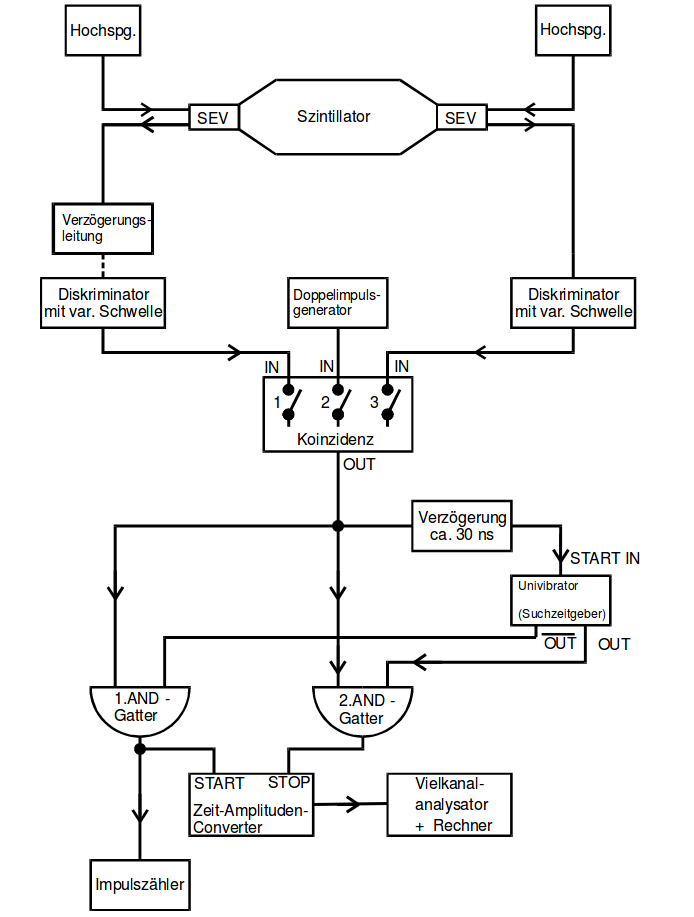
\includegraphics[width=\textwidth]{img/aufbau.png}
  \caption{Schematischer Aufbau der Messapparatur \cite{FP}}
  \label{aufbau}
\end{figure}

Der Diskriminator in \autoref{aufbau} dient dazu, Dunkelpulse zu filtern. Diese Dunkelpulse werden durch thermische Bewegung von Elektronen ausgelöst und besitzen in der Regel eine geringere Amplitude als Photonenpulse. Um keine echten Pulse zu verlieren, wird die Schwelle, bei der Pulse durchgelassen werden, nicht zu hoch eingestellt. Aufgrund der endlichen Ausbreitungsgeschwindigkeit des Lichts im Tank, kann ein Puls zeitversetzt an den beiden SEVs ankommen. Außerdem ist die Laufzeit der Signale nicht identisch. Deshalb wird die Breite des Diskriminators so eingestellt, dass ein Signal trotz dieses Zeitversatzes als koinzidentes Ereignis erkannt wird. Als weiterer Filter wird eine Koinzidenz verwendet; nur wenn ein Signal von beiden SEVs eintrifft, wird es als Myonsignal akzeptiert, da die Wahrscheinlichkeit, in beiden SEVs gleichzeitig einen Dunkelpuls zu messen, gemäß einer Poissonverteilung abnimmt.

Zur Einstellung der richtigen Diskriminatorschwelle wird zunächst ein Zählwerk angeschlossen und die beiden SEVs werden so eingeregelt, dass in beiden Kanälen jeweils eine Rate von 20 bis 40 pro Sekunde gemessen wird. Dazu werden die Breite und die Höhe des Diskriminators, sowie die Länge der Verzögerungsleitungen zwischen SEV und Diskriminator eingestellt. Daraufhin wird die Koinzidenz eingestellt, dass die Suchzeit maximal ist, ohne dass die Zählrate durch Untergrundereignisse dominiert wird. Der TAC wird mit Hilfe eines Doppelpulsgenerators kalibriert; die Pulse werden mit einer Frequenz von $\SI{1}{\kilo\hertz}$ erzeugt und die Linearität zwischen dem Abstand der Pulse und der Amplitude der resultierenden Spannnung gezeigt. Die eigentliche Messung wird über mindestens 24 Stunden durchgeführt, um eine ausreichende Statistik zu erhalten, außerdem wird zum Ende der Messung notiert, wie viele Startpulse ohne Stoppulse und wie viele Startpulse mit Stoppulsen an den Impulszählern jeweils aufgetreten sind.

\FloatBarrier
